\section{Trade-offs}
\subsection{Circuit overhead}
Let $p$ be the probability that Tor Browser submits an SFO to a sampled CTR on a
fresh independent circuit, and $\mathcal{D}$ a distribution that describes how
many SFOs are presented on a website visit.  As shown in
Equation~\ref{eq:sub-oh}, we can now estimate the resulting circuit overhead.
\begin{equation} \label{eq:sub-oh}
	f(p,\mathcal{D}) =
		\frac{p}{n} \sum_{i=1}^{n} c_i, \textrm{where } c_i\sample\mathcal{D}
\end{equation}

We decided to approximate $\mathcal{D}$ using the most frequently viewed reddit
pages as of December 4, 2019.\footnote{%
	\url{https://github.com/pylls/padding-machines-for-tor/commit/353bfa75e9f7d6aa0a1dff9516ff234cbf0f4562}
} This was motivated by the intuition that such web pages should include more
resources than basic front pages, such that $\mathcal{D}$ is more likely to be
overestimated rather than underestimated.  Further, we are likely not
underestimating $\mathcal{D}$ because these SFOs were collected using fresh
Chromium instances that call home on start-up, thereby generating a few
additional SFOs per data point that were left \emph{unfiltered} in our data set.

% TODO: replace 'z' with concrete number from our data set
Using $p=\frac{1}{10}$ and plugging our approximated $\mathcal{D}$ into
Equation~\ref{eq:sub-oh}, the resulting circuit overhead is $z$.  It should be
noted that these circuits are \emph{light} in terms of bandwidth when compared
to loading an entire website.

\begin{figure}
	\centering
	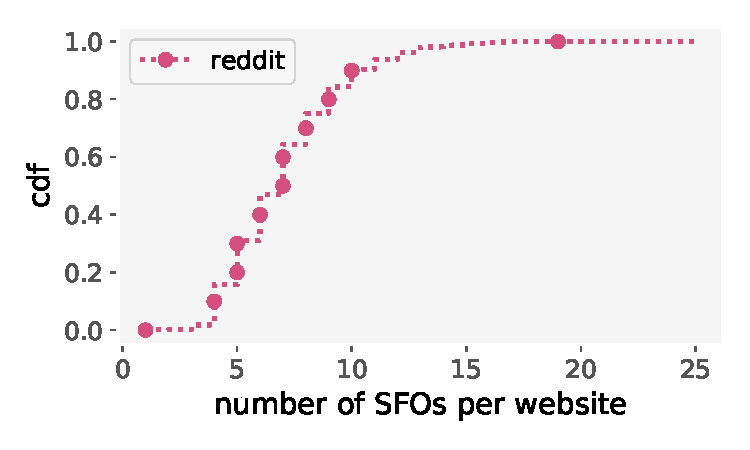
\includegraphics[width=\columnwidth]{../exp/plot/img/sfo-dist}
	\caption{%
		SFO distribution derived from the most frequently viewed reddit pages as
		of December 4, 2019.
	}
	\label{fig:sfo-dist}
\end{figure}
